\chapter{Die Konstruktionalisierung von [Definitartikel\,+\,N]} \label{bicpic}

In Abschnitt \ref{sec:konstruktionalisierung} der Arbeit wurde dafür argumentiert, dass die Entwicklung des Definitartikels einen Konstruktionalisierungsprozess darstellt: Ein Form-Funk"-tions"-paar etabliert sich als neuer Knoten im Konstruktionsnetzwerk. Mit der Korpusuntersuchung wurden die drei zentralen Variablen dieser Konstruktionalisierung beleuchtet -- das funktionale Spektrum von \object{dër}, die kategoriale Füllung des N-Slots sowie der Status der gesamten Struktur im sich wandelnden NP-System des Althochdeutschen. Im vorliegenden Kapitel werden diese Ergebnisse nun genutzt, um den diachronen Werdegang von [\object{dër}\,+\,N] vor dem Hintergrund eines gebrauchsbasierten Modells zu rekonstruieren. 
Der Fokus liegt damit auf dem Prozess der Konstruktionalisierung. Es bleibt zukünftigen Studien überlassen, die Analysen in (formale) Entwürfe eines ahd. Konstrukionsnetzwerkes zu integrieren und  mit späteren Entwicklungsstufen der Konstruktion in Verbindung zu bringen. 

In \ref{diskussion:der} erfolgt zunächst eine Diskussion zum kategorialen Wandel von \object{dër}.  In Abschnitt \ref{sec:disk-expansion} wird ein mehrdimensionales Expansionsmodell basierend auf den Faktoren Belebtheit,  Individualität und Agenitivität vorgeschlagen. Anschlies\-send wird in Abschnitt \ref{sec:disk-ana-entrench} die Netzwerk-Perspektive eingenommen, indem Ana"-lo"-gie- und Entrenchmentprozesse betrachtet werden, die begünstigend oder auch blo"ckierend auf den Wandel eingewirkt haben. 

\section{Der funktionale Wandel von \object{dër}} \label{diskussion:der}

In den meisten diachron angelegten Untersuchungen zur Entwicklung des Definitartikels geht es um die Frage, ob und zu welcher Zeit ein ursprüngliches Demonstrativum als Definitartikel klassifiziert werden kann. Mögliche Antworten für den deutschen Definitartikel liefert Abschnitt \ref{sec:abwann}. Anschließend werden in Abschnitt \ref{sec:disk-bruecken} Sprachdaten diskutiert, die  als Brückenkontexte für den Übergang von pragmatischen zu semantischen Definitheitskontexten vorgeschlagen werden. Abschnitt \ref{sec:disk-entwicklung} stellt eine neue, aus den Daten abgeleitete Version des Grammatikalisierungspfades vor. 

\subsection{Ab wann ist \object{dër} ein Definitartikel?}\label{sec:abwann}

Die Frage, ab wann man in der deutschen Sprachgeschichte davon ausgehen kann, dass sich das ursprüngliche Demonstrativum \object{dër} zum Definitartikel gewandelt hat, ist nicht eindeutig zu beantworten -- zu heterogen ist die Datenlage und zu vielseitig sind die Kriterien, die den Artikelstatus rechtfertigen. Dennoch kann man aus den Ergebnissen der vorliegenden Untersuchung eine Annäherung wagen. 

Die Korpusuntersuchung hat offengelegt, dass \object{dër} bereits in den frühesten Texten äußerst frequent auftritt und als typischer Einleiter für definite Phrasen fungiert. Die hohe Frequenz und breite Kombinierbarkeit mit unterschiedlichen Substantivtypes ist ein wichtiges Indiz dafür, dass das ursprüngliche Demonstrativum schon zu Beginn der althochdeutschen Überlieferung über eine breite funktionale Spannweite verfügt. Auch die Tatsache, dass sich mit \object{dëser} bereits ein neuer Demonstrativartikel herausgebildet und der Definitheitszyklus \parencite{Greenberg1978,vanGelderen2007} von Neuem eingesetzt hat, spricht dafür, dass \object{dër} funktional breiter geworden ist und seinen Platz als prototypisches Demonstrativum allmählich räumt \parencite[ähnlich auch][]{Schlachter2012}: Schon im Isidor ist nicht \object{dër}, sondern  \object{dëser} das bevorzugte Mittel, um unmittelbare anaphorische Referenzbezüge im Text herzustellen \parencite[139]{Oubouzar1989}. Und diese gehören bekanntermaßen zum Hauptarbeitsfeld von Demonstrativa  \parencite{Diessel1999}. Die Analysen zu Otfrids Evangelienbuch weisen ebenfalls darauf hin, dass die beiden Artikelwörter sich die Definitheitskontexte aufteilen: Während \object{dëser} nur in pragmatisch-definiten Kontexten auftritt, dienen \object{dër}-Phrasen fast ausschließlich zum Ausdruck von semantischer Definitheit. 

Für definite Gebrauchskontexte, in denen Sprecherinnen und Sprecher von Artikelsprachen einen Artikel setzen \herkur{müssen} \parencite[832]{Himmelmann2001}, finden sich bereits in den frühesten Schriftstücken  \object{dër}-Belege. Dies wurde insbesondere an Superlativen deutlich, die schon im Isidor, dem ältesten Text der Untersuchung, mit \object{dër} auftreten. Sie sprechen dafür, dass das genuine Demonstrativum seine funktionale Reichweite bereits im frühen Althochdeutschen in Richtung semantische Definitheit ausgebaut hat. Mit der Stichprobenanalyse (zufällige Auswahl von 100 NPs) wurden in den drei untersuchten Schriftstücken (Isidor, Tatian und Otfrid) Belege von [\object{dër}\,+\,N] in abstrakt-situativen Definitheitskontexten nachgewiesen, also den Definitheitskontexten, die mit Definitartikel, aber nicht mit Demonstrativa markiert werden können. Dabei nimmt der Anteil von determinierten zu undeterminierten Phrasen diachron zu: Im Isidor sind es ungefähr ein Fünftel, im Tatian ein Drittel und bei Otfrid die Hälfte. Für Notker steht eine solche Kontextanalyse noch aus. Es ist zu erwarten, dass hier der Anteil an \object{dër}-Phrasen noch größer ist. Hierfür sprechen die Analysen von Oubouzar, die bei Notker keine semantischen Restriktionen mehr für den Gebrauch von \object{dër} sieht \parencite[573]{Oubouzar1989}.\footnote{Eine Ausnahme sind Prädikative wie \object{Er ist der Lehrer}.} Ihre Beobachtungen werden durch die vorliegende Korpusuntersuchung gestützt. Nicht nur Superlative, sondern auch Unika werden bei Notker regelmäßig mit \object{dër} determiniert. Spätestens zu dieser Zeit kann man daher -- gemessen an der funktionalen Spannbreite -- \object{dër} den Status eines Definitartikels zuschreiben. 

Die Stichprobenanalyse hat darüber hinaus auch Belege für generische Ausdrücke mit \object{dër} zu Tage gefördert. Dies ist insbesondere für den Isidor bemerkenswert, da bislang davon ausgegangen wurde, dass in diesem frühen Text generische Ausdrücke ausschließlich in Form von blanken Nomen erscheinen \parencites()()[80]{Oubouzar1992}[145]{Kraiss2012}. Auch im etwas jüngeren Monseer Matthäus, der in der vorliegenden Untersuchung nicht Teil der Stichprobenanalyse war, finden sich \textcite{Hodler1954} zufolge bereits generische Referenzen mit \object{dër} (vgl. Abschnitt \ref{sec-generisch}). Somit gehört der generische Gebrauch schon seit dem frühen Althochdeutschen zum Arbeitsgebiet von [\object{dër}\,+\,N].  Allerdings verläuft die Durchsetzung hier viel zögerlicher als in anderen semantischen Definitheitskontexten. Bis heute können generische Phrasen im  Plural auch ohne Definitartikel auftreten, vgl. \object{(die) Pandabären sind vom Aussterben bedroht} \parencite[][145]{Barton2015}. Zudem wird neben dem Definitartikel auch der Indefinitartikel als Generizitätsmarker genutzt \parencite{Petrova2020}.

Mit der Untersuchung konnte also nachgewiesen werden, dass \object{dër} schon im frühen Althochdeutschen viel mehr ist als lediglich ein funktionales Aquivalent zum heutigen Demonstrativartikel, wie es u.a. von \textcite{Philippi1997} und \textcite{Demske2001} postuliert wird. Der Ausschnitt des Althochdeutschen, der uns über die Überlieferungen gegeben ist, setzt demnach erst ein, nachdem \object{dër} schon in für Demonstrativa untypische Kontexte eingedrungen ist. 


\subsection{Brückenkontexte}\label{sec:disk-bruecken}

In Abschnitt \ref{sec:bruecke} wurden der anaphorische und der anamnestische Gebrauch als Brückenkontexte gehandelt. Beide Typen sind in den Daten belegt, wenn auch nicht besonders häufig (vgl. die Zahlenwerte zu den ambigen Fällen in Abschnitt \ref{sec:ergeb-defkontexte}). Bezüglich der Frage, wie der funktionale Wandel von Demonstrativ- zu Definitartikel vonstatten geht, sind ambige Fälle, die sich zwischen pragmatisch-definiter und semantisch-definiter Lesart bewegen, besonders interessant, da sich an ihnen die Reanalyse zum Definitartikel rekonstruieren lässt. Sie werden nachfolgend an Beispielen\footnote{In den untersuchten Daten sind diese Fälle als \hervor{ambig} annotiert, s. Trolling (Todo: URL und Namen der Daten nennen)} illustriert. 

 
%\subsubsection{Zwischen anaphorischem und abstrakt-situativem Gebrauch}

Die Korpusuntersuchung hat \object{dër}-Belege zum Vorschein gebracht, die auf den ersten Blick wie einfache anaphorische Wiederaufnahmen aussehen. In diesen Fällen befand sich ein vorausgehender koreferenter Ausdruck in der unmittelbaren Textumgebung. Allerdings leitete die Wiederaufnahme -- wie sonst bei Demonstrativa häufig (s. Abschnitt \ref{sec:anaphorisch}) -- keinen Topikwechsel ein. Entweder ist der Referent bereits eindeutig als Topik etabliert worden. Dies ist besonders gut an \object{heilant} zu sehen, der im Tatian fast immer mit \object{dër} wiederaufgenommen wird. Oder es gibt kein explizites Abgrenzungsmoment zu anderen potentiellen Referenten.
In diesen Fällen \hervor{braucht} der Rezipient das Antezedens nicht mental zu aktivieren, damit die eindeutige Referenz glückt. Die Identifizierung kann auch über das Weltwissen erfolgen, s. Beispiel \REF{ex:I2245} aus dem Isidor. Die Phrase \object{oba} \object{dhem} \object{uuazsserum} bezieht sich auf ein kurz zuvor genanntes Bibelzitat \object{endi gotes gheist suueiboda oba uuazsserum} (I. 4,4).

% basiert auf
%\begin{exe}
\ex \label{ex:I2245} \gll \object{In dhiu} \object{auh} \object{dhanne} \object{,} \object{dhazs} \object{ir} \object{oba} \object{dhem} \object{\underline{uuazsserum}} \object{suueiboda} \object{,} \object{dhen} \object{heilegun} \object{gheist} \object{dhar} \object{bauhnida} \object{. } \\
{dabei} {auch} {damals} {} {dass} {er} {auf} {der} {Wasser} {sich bewegen} {} {der} {heilig} {Geist} {da} {zeigen} {}\\
\glt TODO: nhd. Übersetzung (I.4,4)
\end{exe}


\begin{exe}
\ex \label{ex:I2245} \gll \object{In dhiu} \object{auh} \object{dhanne}, \object{dhazs} \object{ir} \object{\textbf{oba}} \object{\textbf{dhem}} \object{\textbf{uuazsserum}} \object{suueiboda}, \object{dhen} \object{heilegun} \object{gheist} \object{dhar} \object{bauhnida}  \\
{dabei} {auch} {dann}, {dass} {er} {auf} {dem} {Wasser} {schwebt}, {den} {heiligen} {Geist} {da} {zeigte}\\
\glt \extrans{Darin, dass er über d(ies)em Wasser schwebte, zeigte sich der heilige Geist} (I 4,4)
\end{exe}

\noindent 
Zwar ist hier  eine demonstrativ-wiederaufnehmende Lesart zugunsten einer höheren Expressivität nicht auszuschließen. Es ist aber auch möglich, die Phrase als \herkur{über dem Wasser} zu übersetzen und damit eine abstrakt-situative Lesart zu erhalten. 


%\subsubsection{Zwischen anamnestischem und abstrakt-situativem Gebrauch}

Das nachfolgende Beispiel illustriert die konzeptuelle Überschneidung von anamnestischer und abstrakt-situativer Lesart: Mit \object{thie geba} wird auf eine Gabe referiert, die einer gläubigen Leserschaft bekannt sein müsste und die mit dem restriktiven Nebensatz in Erinnerung gerufen wird. Der Relativsatz fungiert dann als \object{aktivierende Modifizierung} \parencite[78f.]{Himmelmann1997}, vgl. hierzu die Ausführungen in Abschnitt \ref{sec:amnamnestisch}. 

%basiert auf
%\begin{exe}
\ex \label{ex:T9827} \gll \object{gisih} \object{thaz} \object{thu} \object{iz} \object{niomanne} \object{ni} \object{quedes} \object{,} \object{ouh} \object{fár} \object{inti} \object{giougi} \object{thih} \object{themo} \object{biscofe} \object{inti} \object{bring} \object{thie} \object{\underline{geba}} \object{thie} \object{thar} \object{gibót} \object{Moyses} \object{ín} \object{zi} \object{giuúiznesse} \object{.} \\
{sehen} {daß} {du} {er} {niemand} {nicht} {sagen} {} {sondern} {fahren} {und} {zeigen} {du} {der} {Bischof} {und} {bringen} {der} {Gnade(ngabe)} {der} {da} {gebieten} {Moses} {er} {zu} {Zeugnis} {}\\
\glt Siehe zu, sage es niemand; sondern gehe hin und zeige dich dem Priester und opfere die Gabe, die Mose befohlen hat, zu einem Zeugnis über sie (T.46,4)
\end{exe}


\begin{exe}
\ex \label{ex:T9827} \gll \object{gisih} \object{thaz} \object{thu} \object{iz} \object{niomanne} \object{ni} \object{quedes} \object{,} \object{ouh} \object{fár} \object{inti} \object{giougi} \object{thih} \object{themo} \object{biscofe} \object{inti} \object{bring} \object{\textbf{thie}} \object{\textbf{geba}} \object{thie} \object{thar} \object{gibót} \object{Moyses} \object{ín} \object{zi} \object{giuúiznesse} \\
{Siehe} {dass} {du} {es} {niemandem} {nicht} {sagst} {} {sondern} {fahre} {und} {zeige} {dich} {dem} {Bischof} {und} {bringe} {die} {Gabe} {die} {da} {gebot} {Moses} {ihn} {zu} {Zeugnis} {}\\
\glt \extrans{Siehe, dass du es niemandem sagst, sondern gehe hin und zeige dich dem Priester und opfere die Gabe, die Moses befohlen hat zu einem Zeugnis über sie.} (T 46,4)
\end{exe}


\noindent 
Der Nebensatz kann aber auch als bloße Identifikationshilfe dienen, um der Leserschaft zu verdeutlichen, um welche Gabe es sich genau handelt, also als \object{etablierende Modifizierung} \parencite[79]{Himmelmann1997}. Die Referenz basiert dann nicht auf der Aktivierung einer spezifischen Erinnerung. Sie gelingt alleine durch den Bezug auf einen durch das Weltwissen bekannten Referenten (hier: \object{Moses}). Der eingeführte Referent (\object{die Gabe}) wird dadurch eindeutig definiert.  In diesem Fall würde der Beleg unter die \object{nicht-familiären} Gebrauchskontexte fallen, in denen nach \textcite{Hawkins1978} nur Definitartikel, aber keine Demonstrativa möglich sind (vgl. Abschnitt \ref{sec:nicht-fam}). 

%\subparagraph*{Die Brücke zum generischen Gebrauch}
%
%Oben wurde gezeigt, dass generische Ausdrücken schon in den frühsten Texten mit \object{dër} auftreten, also noch bevor der Gebrauch in den semantisch-definiten Kontexte zur Regel wurde. Der Brückenkontext von referentiell-definiter zu nicht-referentiell-generischem Gebrauch sollte daher bei den pragmatischen Definita gesucht werden. Der nachfolgende Beleg aus dem Isidor könnte sowohl generisch als auch anamnestisch interpretierbar sein und deswegen ein möglichen Brückenkontext abbilden. %
%\begin{exe}
\ex \label{ex:I4134} \gll \object{Dhiz} \object{ist} \object{dhiu} \object{sahha} \object{christes} \object{chiburdi} \object{0} \object{dhen} \object{\underline{iudeoliudi}} \object{0} \object{dhoh} \object{sie} \object{inan} \object{chiboranan} \object{chilauben} \object{0} \object{lastront} \object{inan} \object{dhoh dhiu huuedheru} \object{in} \object{cruci} \object{chislaganan} \object{endi} \object{dodan} \object{. } \\
{dieser} {sein} {der} {Ursache} {Christus} {Geburt} {} {der} {Juden} {} {doch} {er} {er} {gebären} {glauben als} {} {verhöhnen} {er} {dennoch} {in} {Kreuz} {schlagen} {und} {tot} {}\\
\glt TODO: nhd. Übersetzung (I.5,11)
\end{exe}


\subsection{Modellierung des Entwicklungspfades}\label{sec:disk-entwicklung}

Es ist deutlich geworden, dass sowohl der anamnestische als auch der anaphorische Kontext leicht von einer anderen Lesart überlagert werden kann, nämlich dem Rückbezug auf das Weltwissen. Der Sprecher oder die Sprecherin kann mit  \object{dër} auf den Referenten, um den es geht, expressiv \hervor{zeigen} -- der Rezipient könnte diese Zeigegeste allerdings leicht \hervor{ignorieren}, wenn der Referent ohnehin eindeutig identifizierbar ist. Umgekehrt kann ein Rezipient \object{dër} als verbale Zeigegeste verstehen, selbst wenn sie vom Sprecher oder der Sprecherin gar nicht intendiert ist.
Der Einsatz von \object{dër} sichert sowohl beim anaphorischen als auch beim anamnestischen Gebrauch das Verständnis und macht deutlich, um welchen Referenten es geht. Je häufiger \object{dër} auf einen Referenten verweist, der auch ohne den Kontext oder den Rückbezug auf eine gemeinsame Erinnerung, sondern über das generelle Wissen etabliert wird, umso mehr rückt die expressive Zeigefunktion in den Hintergrund. Für immer mehr Diskursteilnehmer wird der nicht expressive Gebrauch zum Normalfall, so dass diese semantisch-definite Lesart nach und nach zum Bestandteil der Konstruktion [\object{dër}\,+\,N] wird. 

Anstatt den anaphorischen und anamnestischen Gebrauch als zeitlich aufeinanderfolgende Gebrauchskontexte  auf dem Grammatikalisierungspfad abzubilden, schlage ich vor, dem funktionalen Wandel vom Demonstrativ- zum Definitartikel eine Phase vorauszuschicken, die diese beiden Kontexttypen gleichermaßen umfasst.\footnote{Es sei angemerkt, dass es theoretisch durchaus möglich ist, dass \object{dër} ursprünglich primär anaphorisch und erst später auch anamnestisch gebraucht wurde. Diese Chronologie lässt sich an den Daten allerdings nicht ablesen.} Darüber hinaus darf auf Basis der Daten ein generischer \hervor{Seitenpfad} angenommen werden, der schon im frühen Althochdeutschen angelegt wird und parallel zur \hervor{Hauptstraße} der Grammatikalisierung innerhalb der referentiell-definiten Kontexte verläuft, s. Abbildung \ref{abb:expansion-definitheit}. Der Pfad basiert auf dem im Theorieteil der Arbeit vorgestellten Modell aus \textcite{Schmuck2014} (s. Abschnitt \ref{sec:stufen}). 

 
\begin{figure}
\begin{center}
  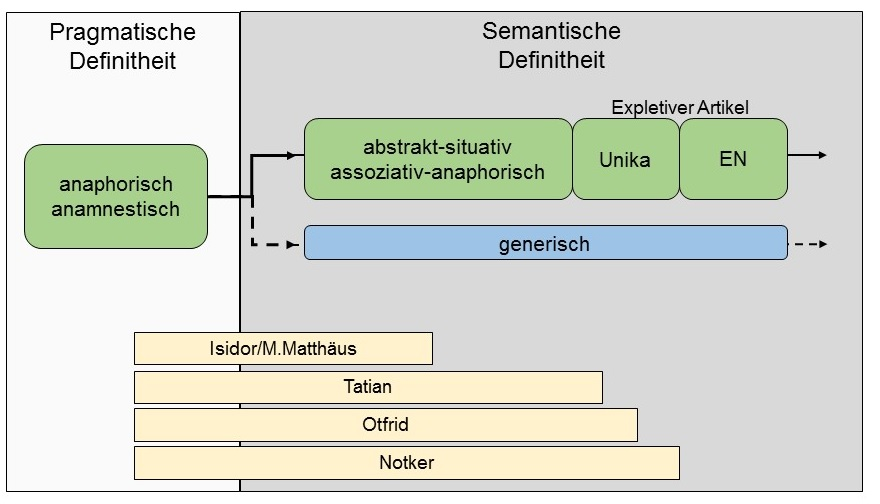
\includegraphics[width=\textwidth]{images/diskussion-generisch-farbe-neu.jpg}
\caption {Entwicklungspfad von [\object{dër}\,+\,N]} 
\label{abb:expansion-definitheit}
\end{center}
\end{figure} 
 
\textcite[105]{Schmuck2014} argumentieren dafür, dass mit der Ausbreitung auf Unika der Weg für den onymischen Artikel geebnet wird, da sich hier eine konzeptuelle Überschneidung finden lässt. Die Frage, wie man den Übergang in Richtung generischen Gebrauch modellieren müsste, ist hingegen noch offen. Es wäre denkbar, dass es Kontexte gibt, in denen eine Aussage über einen zuvor im Text oder Diskurs erwähnten Referenten gemacht wird, die auch generisch interpretierbar ist, z.B. die Referenz auf eine bestimmte Gruppe, über die eine allgemeine Aussage gemacht wird, etwa: \object{Diese/Die Heiden glauben nicht an Jesus}. 

Auf Basis der Korpusuntersuchung sowie unter Bezugnahme auf bisherige Forschung\footnote{Für den Tatian hat die Stichprobenuntersuchung bspw. keinen Beleg für eine generische Referenz mit \object{dër} hervorgebracht. \textcite{Oubouzar1992} hat diesen Gebrauchstypus allerdings eindeutig nachgewiesen, vgl. ausführlich Abschnitt \ref{sec-generisch} der vorliegenden Arbeit.} können die untersuchten Textdenkmäler in diesem Entwicklungspfad verortet werden. Wie man in Abbildung \ref{abb:expansion-definitheit} sieht, übernimmt  \object{dër} in allen Texten bereits Aufgaben aus der Domäne des Definitartikels, d.h. der semantischen Definita. Die Unika sind bereits im Tatian und noch häufiger auch bei Otfrid in \object{dër}-Phrasen zu finden. Das \object{dër} bei Notker steht bereits an der Schwelle zu den Eigennamen, da es hier vereinzelt schon als syntaktisch motivierter Artikel auftritt \parencite[\object{der einrihtigo cato} \extrans{der unbeugsame Cato}, s.][638]{Oubouzar1989}.

Die eigentliche Expansionsphase für den onymischen Artikel setzt allerdings erst im Frühneuhochdeutschen ein \parencite{Schmuck2020}. 


\section{Expansionspfade von [\object{dër}\,+\,N]} \label{sec:disk-expansion}

Der funktionale Wandel von \object{dër}, der im vorhergehenden Abschnitt aufgezeigt wurde, spiegelt die von \textcite[32--33]{Himmelmann2004} postulierte \object{semantic-prag\-mat\-ic context expansion}. Neben diesem Expansionspfad beschreibt Himmelmann zwei weitere Richtungen, in die sich das Demonstrativum auf seinem Weg zum Definitartikel ausbreiten kann: Die \object{host-class expansion}, also die Ausbreitung von [\object{dër}\,+\,N] auf neue semantische Substantivklassen und die \object{syntactic context expansion}, d.h. die Ausbreitung von zentralen zu weniger zentralen Argumentpositionen \parencite[32--33]{Himmelmann2004}, vgl. Abschnitt \ref{sec:parameter}. Mit den Ergebnissen aus der Korpusuntersuchung können diese groben Stufen der Kontextexpansion weiter ausdifferenziert werden.  

\subsection{Host-class expansion}

Eine der zentralen Hypothesen, die im Theorieteil der Arbeit formuliert wurde, lautet, dass die kontinuierliche Ausbreitung von [\object{dër}\,+\,N] auf neue Substantivklassen (\object{host-class expansion}) belebtheitsgesteuert verläuft. Es wurde ein recht breites Belebtheitskonzept zugrunde gelegt: Die Hauptstufen \textsc{menschlich > belebt > unbelebt} wurden auf Basis der aus der Forschung bekannten Belebtheitshierarchien \parencite[u.a.][]{Comrie1989,Yamamoto1999,Croft2006,Enger2011} am unteren (\hervor{unbelebten}) Ende der Skala um Abstrakta und Massennomen erweitert. Diese weisen nicht nur konzeptuell eine maximale Entfernung zum Menschen auf, sondern verfügen auch über einen geringen Individualitätsgrad. Da sich diese Eigenschaften nur schlecht mit dem emergierenden Definitartikel in seiner Rolle als Individualisierer (s. Abschnitt \ref{sec:individualisierer}) und Marker für Diskursprominenz (s. Abschnitt \ref{sec:kata}) vertragen, gehört diese Substantivklasse zur letzten Bastion des appellativen Wortschatzes, die sich der obligatorischen Definitheitskennzeichnung widersetzt. Zudem korreliert der Faktor (kulturelle) Relevanz (Abschnitt \ref{sec:relevanz}) mit einem hohen Belebtheitsgrad. 

Die Ergebnisse der Korpusuntersuchung haben gezeigt, dass die \object{host-class expansion} tatsächlich belebtheitsgesteuert verläuft. Eine schematische Zusammenfassung bietet Abbildung \ref{abb:expansion-belebtheit}. Sie beruht auf den Ergebnissen aus den Abschnitten \ref{sec:ergeb-definitheit} und \ref{sec:ergeb-belebtheit}. Je intensiver die Farbe, umso stärker ist die Präferenz bzw. die Ablehnung der Konstruktion gegenüber der jeweiligen Kategorie. 

\begin{figure}
\begin{center}
  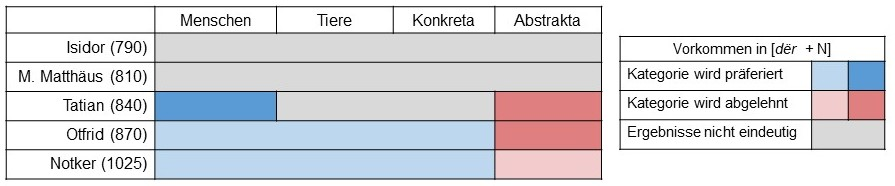
\includegraphics[width=\textwidth]{images/belebtheitsexpansion-neu.jpg}
\caption {Expansion von [\object{dër}\,+\,N] entlang der Belebtheitskala} 
\label{abb:expansion-belebtheit}
\end{center}
\end{figure} 
  
In den frühesten Denkmälern -- dem Isidor und dem Monseer Matthäus -- ist noch kein signifikanter Einfluss der Belebtheit zu beobachten. Allerdings lässt sich an den Daten zum Monseer Matthäus zumindest die Tendenz erkennen, dass belebte Referenten eher determiniert werden als abstrakte, während im älteren Isidor auch Abstrakta zu \object{dër} tendieren. Eine Erklärung könnte im Faktor Relevanz liegen, der durch die Inventur der häufigsten Lemmata mit und ohne \object{dër} aufgedeckt werden sollte:  Im Isidor steht die Determinierung im Dienste einer eindeutigen Argumentationsführung. Dabei werden sowohl zentrale biblische Referenten regelmäßig mit \object{dër} ausgestattet (\object{forasago, magad}) als auch abstrakte (\object{drinissa}). Im Monseer Matthäus sind es vor allem Referenten, die in den Herrschaftsstrukturen zur Zeit Jesus an der Spitze stehen (\object{ewawart, herizoho, herizo}). Im Tatian begünstigt nicht nur die kulturelle Wichtigkeit die Determination, sondern vor allem das Merkmal [+menschlich]. So stehen bspw. \object{heilant, keisar, grafo} regelmäßig mit \object{dër}. Interessanterweise scheint im Tatian und bei Notker auch das Geschlecht eine Rolle zu spielen. Der Anteil an \object{dër}-Phrasen fällt bei weiblichen Referenten niedriger aus als bei männlichen; bei Otfrid ist die Verteilung allerdings genau umgekehrt.

Andere belebte und konkrete Referenten zeigen im Tatian keine Präferenz hinsichtlich der Determination. Abstrakta bleiben hingegen signifikant häufiger undeterminiert. Bei Otfrid und Notker treten auch Tiere und Konkreta präferiert mit \object{dër} auf. In diesen Texten sind außerdem die Schnitte zwischen den Belebtheitskategorien weniger scharf, so dass man schließen kann, dass die \object{dër}-Setzung innerhalb der obersten Belebtheitsstufen zu dieser Zeit schon generalisiert wurde. Für Massenomen hat die Untersuchung nur Einzelbelege mit \object{dër} hervorgebracht, so dass keine Expansion in diesen Bereich nachgewiesen werden konnte.  

Aus dem empirischen Befund für das Althochdeutsche lassen sich drei implikative Expan"-sions"-stadien modellieren, s. \REF{ex:belebtheitsskala}. Implikativ meint Folgendes:  
Wenn eine Sprache Appellativa der dritten Ebene regelmäßig mit Definitartikel ausstattet, ist anzunehmen, dass auch Appellativa aus der zweiten und ersten Ebene obligatorisch determiniert werden; das zweite Stadium impliziert das erste. Die Skala müsste an weiteren Sprachen überprüft werden.  

\begin{exe}
	\ex \label{ex:belebtheitsskala} (Kulturell) relevante und menschliche Referenten (1)\\>  belebte und unbelebte Konkreta (2)\\> Abstrakta und Massennomen (3)
	\end{exe}


\subsection{Syntactic-context expansion} \label{sec:syn-expansion}

Für die \object{syntactic-context expansion} nennt \textcite{Himmelmann2004} zwei Phasen: Zunächst erfasst der emergierende Artikel zentrale Satzglieder (Subjekt oder Objekt), später auch weniger zentrale Argumente, d.h. solche, die formseitig als \hervor{adpositional expressions} realisiert werden, darunter Präpositionalobjekte und Adverbiale \parencite{Himmelmann1998}. In Abschnitt \ref{sec:partizipanten} wurde diese Art der Expansion mit der semantischen Rolle in Verbindung gebracht; sie ist also  die Folge einer semantischen Expansion. Während die Subjekts- und Objektsposition meist zentralen Patizipanten einer Situation entsprechen, werden weniger zentrale (und meist fakultative) Partizipanten als Adverbiale realisiert \parencite{Lehmann2004a}. 

In der Untersuchung wurden formale Kriterien genutzt, um sich dieser Partizipanten"=Opposition zu nähern und zwar, indem alle Präpositionalphrasen in den Blick genommen wurden. Es hat sich gezeigt, dass die Struktur [Präp\,+\,N] zahlenmäßig in allen Denkmälern deutlich gegenüber [Präp\,+\,\object{dër}\,+\,N] dominiert. Eine diachrone Ausweitung lässt sich an den Daten jedoch nicht eindeutig nachweisen, da der Anteil an determinieren Phrasen vom ältesten bis zum jüngsten Text nicht linear zunimmt. Eine Ausweitung des Definitartikels auf Präpositionalphrasen muss also zu einem späteren Zeitpunkt in der Sprachgeschichte einsetzen. 

Darüber hinaus wurde qualitativ vorgegangen und 100 NPs im Isidor, Tatian und Otfrid in Agens und Nicht-Agens eingeteilt. Es zeigt sich, dass die Agens-Belege stärker zur \object{dër}-Setzung tendieren als die Nicht-Agens-Fälle. In den zwei jüngeren Texten ist dieser Unterschied auch signifikant. Die Daten weisen darauf hin, dass die Merkmalskombination [+Agens] und [+(über-)menschlich] am häufigsten eine Determinierung auslösen. In zukünftigen Studien könnte dieser Hypothese mit der Analyse größer Datenmengen auf den Grund gegangen werden. Interessant wäre in diesem Zusammenhang auch, wie die Variablen Belebtheit und \object{dër}-Setzung bei anderen semantischen Rollen ausgeprägt sind, etwa beim Patiens, das sowohl mit belebten als auch mit unbelebten Referenten besetzt werden kann.   

\section{Analogien und Entrenchment im NP-Netzwerk} \label{sec:disk-ana-entrench}

Die Entwicklung des Definitartikels wird von strukturellen Umbauprozessen auf phrasaler Ebene begleitet. Mit der Korpusuntersuchung wurden die Anfänge dieser Prozesse offengelegt. Die Ergebnise können jetzt genutzt werden, um Schematisierungsprozesse abzuleiten und analogische Relationen im NP-Kon"-struktions"-netzwerk zu modellieren. In Abschnitt \ref{sec:disk-schema} wird die Konstruktionalisierung von [Definitartikel\,+\,N] vor dem Hintergrund eines sich etablierenden Determiniererschemas beleuchtet. Gegenstand von Abschnitt \ref{sec:disk-weg-block} sind mögliche \hervor{Wegbereiter} und \hervor{Blockaden}, die den Wandel beeinflusst haben.  

\subsection{Determiniererschema} \label{sec:disk-schema}

In den vorherigen Abschnitten wurde gezeigt, wie sich der Definitartikel durch die einzelnen Definitheitskontexte arbeitet und immer mehr Substantivklassen erfasst. Diese Expansion verdeutlicht, dass sich [\object{dër}\,+\,N] im Laufe des Althochdeutschen von einer Demonstrativ- zu einer Definitartikelkonstruktion wandelt. 
Wie in Abschnitt \ref{sec:entrenchment} erläutert wurde, kann man davon ausgehen, dass mit diesem Wandel ein Entrenchment-Prozess einhergegangen ist: Die Kombination mit immer neuen Substantiv-Types  sorgt für die kognitive Verfestigung des Schemas [Definitartikel\,+\,N], welches dazu dient, definite Referenten zu kennzeichnen, s. Abbildung \ref{abb:entrenchment-ther}. 

\begin{figure}
\begin{center}
  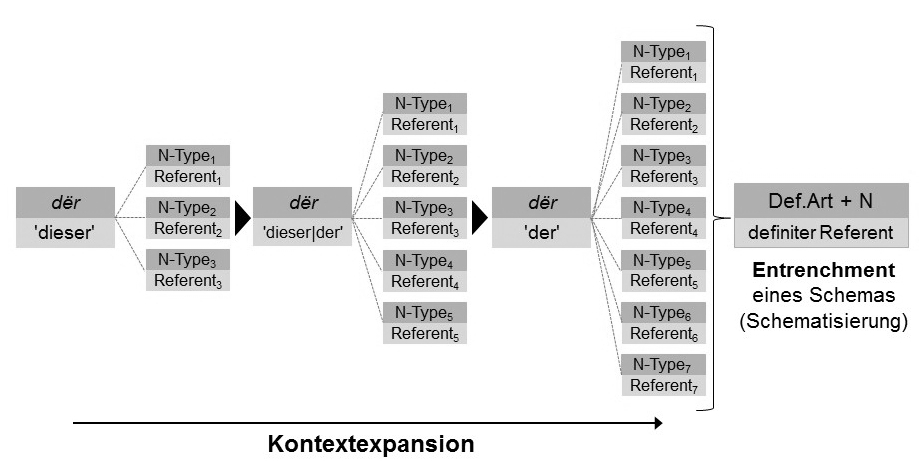
\includegraphics[width=12cm]{images/entrenchment-def-N-neu-sw.jpg}
\caption {Herausbildung eines Definitartikelschemas} 
\label{abb:entrenchment-ther}
\end{center}
\end{figure} 

Die Korpusuntersuchung dokumentiert, wie \object{dër} nach und nach an Gebrauchsfrequenz gewinnt und damit die Determiniererposition besetzt (vgl. Abschnitt \ref{sec:ergeb-ther-freq}). Dies geschieht zu Lasten von anderen pränominalen Determinierern. Die \hervor{Leittragenden} sind vor allem die pränominalen Genitivattribute, welche an den rechten Rand der Phrase gedrängt werden \parencite[zur weiterführenden Diskussion s.][]{Demske2001}. Und andererseits die Possessivartikel -- die  Referenten aus der Klasse der Körperteile an \object{dër} abtreten (s. Abschnitt \ref{sec:ergeb-belebtheit}). 

Die Proxy-Suche nach NP-Strukturtypen (s. Abschnitt \ref{sec:ergeb-np-struktur}) hat offengelegt, dass der nominale Kopf bereits im frühen Althochdeutschen (im Isidor) in ca. der Hälfte der Belege von einem pränominalen Element begleitet wird. Bei der Mehrzahl handelt es sich um definite Einleiter -- neben dem ursprünglichen Demonstrativum \object{dër}, sind es Possessiva, demonstratives \object{sëlb} oder \object{dëser} sowie Genitivattribute. Man kann schlussfolgern, dass Sprecherinnen und Sprecher auf Basis dieser unterschiedlichen Determinierertypen ein übergeordnetes Schema abstrahieren, bestehend aus einem definiten pänominalen Slot\,+\,N \parencite[ähnlich fürs Altenglische][]{Sommerer2011}. 
  
\begin{figure}
\begin{forest} for tree = {edge={thick,dashed},grow=west,child anchor=parent}
% %   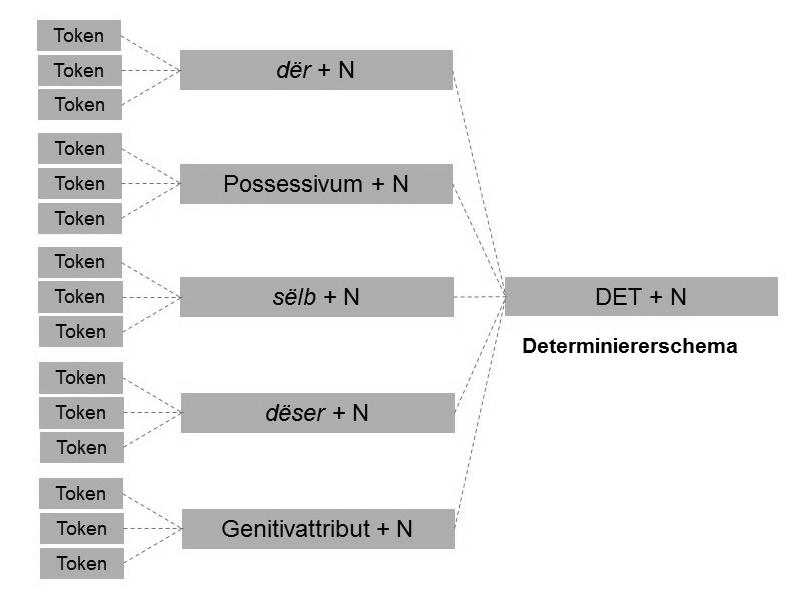
\includegraphics[width=10cm]{images/schematisierung-det-slot-sw.jpg}
[DET\,+\,N\\Determiniererschema,align=center,name=det,l sep=1cm,
  [\textit{dër}\,+\,N [Token,tier=token] [Token,tier=token] [Token,tier=token]]
  [Possessivum\,+\,N [Token,tier=token] [Token,tier=token] [Token,tier=token]]
  [\textit{sëlb}\,+\,N [Token,tier=token] [Token,tier=token] [Token,tier=token]]
  [\textit{dëser}\,+\,N [Token,tier=token] [Token,tier=token] [Token,tier=token]]
  [Genitivattribut\,+\,N [Token,tier=token] [Token,tier=token] [Token,tier=token]]
]
\end{forest}
\caption {Herausbildung eines Determiniererschemas\label{abb:schematisierung}}
\end{figure}
 
Der gemeinsame Nenner für die Besetzung des Slots ist die definite Bedeutungskompente. Das ursprüngliche Demonstrativum ist ein guter Kandidat, um diesen Slot regelmäßig zu besetzen. Im Vergleich zu \object{dëser} oder \object{sëlb} hat es eine viel generelle Bedeutung und anders als ein Possessivum oder Genitivattribut setzt sein Gebrauch nicht notwendigerweise eine Besitzrelation oder sonstige Zugehörigkeit voraus. Das Funktionsspektrum von \object{dër} hat also die größte Reichweite, was die  Kombinierbarkeit mit unterschiedlichen N-Types begünstigt.

Wichtig für die Herausbildung des Determiniererschemas sowie die Obligatorisierung von \object{dër} in pränominaler Position ist auch die Frage der Stellungsfestigkeit. Die Korpusuntersuchung hat offengelegt, dass die Voranstellung der Determinierer (neben \object{dër} wurden Possessiva und Indefinita wie \object{ein} oder \object{sum} untersucht, s. Abschnitt \ref{sec:ergeb-np-struktur}) in allen Texten klar dominiert. Die meisten Nachstellungen finden sich bei Otfrid. Da dies der einzige poetische Text ist, lassen sich diese Fälle auf metrische Erfordernisse zurückführen. Neben der Stellung ist auch die Anzahl der Phraseneinleiter schon in den frühesten Texten stark reguliert. Fälle, in denen zwei flektierende Determinierer gleichzeitig vor einem Bezugsnomen stehen, sind nur vereinzelt belegt. Auch die Struktur [Artikelwort\,+\,pränominaler Genitiv\,+\,N] ist sehr selten und kommt nur im ältesten Text mit knapp 2\% auf der Liste der zehn häufigsten Strukturtypen vor. Für den jüngsten Text, Notkers Boethius, hat die Untersuchung keine solche Phrasen dokumentiert. Die zunehmende Abwanderung des attributiver Genitive an die postnominale Position sorgt zusätzlich dafür, dass der linke, phraseneinleitende Slot die \object{Default}-Position für flektierende Elemente wird. Aus der Tatsache, dass die pränominalen Elemente in Bezug auf Kasus-, Genus- und Numerusinformationen mit ihrem Bezugsnomen übereinstimmen, kann man ableiten, dass Sprecherinnen und Sprecher die Phraseneinleiter als eigene, auf formaler Analogie basierende Kategorie begreifen und sich eine schematische Konstruktion [flektierender Phraseneinleiter + N] kognitiv einschleift. Die Schematisierung steht im Dienste des klammernden Verfahrens \parencite{Ronneberger-Sibold1994,Ronneberger-Sibold2010a,Szczepaniak2010,Szczepaniak2011a,Flick2018}. Man kann davon ausgehen, dass die paradigmatische Einbindung in die Klasse der Phraseneinleiter sich positiv auf die Obligatorisierung von [\object{dër} + N] auswirkt.     


\subsection{\hervor{Wegbereiter} und \hervor{Blockaden}} \label{sec:disk-weg-block}

Die Korpusuntersuchung hat gezeigt, dass in allen Texten eine klare Korrelation zwischen schwach deklinierten Adjektiven und \object{dër}-Setzung vorliegt. Die Korrelation ist semantisch begründet: Ein schwach flektiertes Adjektiv sorgt für eine individualisierende Lesart des Bezugsnomens (vgl. hierzu ausführlich Abschnitt \ref{sec:flexion}). Die Kombination mit \object{dër} unterstreicht diese Lesart zusätzlich.  Die einzelnen Elemente der NP sind aber nicht nur semantisch miteinander verknüpft, sondern auch über ihre formalen Merkmale. Denn sowohl das Artikelwort als auch das Adjektiv und das Bezugsnomen stimmen in Kasus, Genus und Numerus überein. Die darauf resultierende kooperative Flexion hilft, Mehrdeutigkeiten, die durch Synkretismen im Flexionssystem entstehen, aufzulösen \parencite[127]{Szczepaniak2010}. Die hohe Frequenz und die enge sowohl semantische als auch morphosyntaktische Verzahnung ist ein Indiz dafür, dass Sprecherinnen und Sprecherinnen die Struktur [\object{dër}\,+\,Adjektiv\textsubscript{schwach} + N] in ihrer Gesamtheit als Schema abspeichern. In diesem syntaktischen Kontext wird der Gebrauch von \object{dër} also schon früh zum Normalfall. Die Schematisierung kurbelt dadurch die Reanalyse des ursprünglich demonstrativen und fakultativen \object{dër} zum obligatorischen Definitheitsmarker an. In dieser Funktion kann das Artikelwort analogisch auf andere Kontexte übertragen werden und so die Entwicklung auf Systemebene vorantreiben. Dass ein schwach flektiertes Adjektiv fast immer die Setzung von \object{dër} zur Folge hat, könnte auch für die Superlativ-Konstruktionen von Bedeutung sein: Das Schema [\object{dër} + Adjektiv\textsubscript{schwach} + N], das sich vor allem auf Formen im Positiv und Komparativ bezieht, könnte analogisch auch auf Superlative ausgeweitet worden sein. Dass die \object{dër}-Setzung vor attributiv gebrauchten Adjektiven im Superlativ etwas häufiger ist als bei den substantivierten Superlativen,  stützt diese Vermutung. 

Aus den Daten lassen sich darüber hinaus auch ganz spezifische Token herausgreifen, die auf ähnliche Weise wie die bisher genannten Schemata dem funktionalen Wandel von \object{dër} dienlich sind und die somit zu \hervor{Wegbereitern} für die Entwicklung werden. Gemeint sind Phrasen wie \object{dër heilant} oder \object{dër ewawart}, die eine hohe Tokenfrequenz aufweisen und daher als eigene Konstruktion abgespeichert werden \parencite[= Token-Entrenchment, s.][]{Ziem2013}. Das Besondere ist, dass diese Konstruktionen zum Ausdruck semantischer Definitheit genutzt werden. So ist mit  \object{dër heilant} im Tatian immer Jesus gemeint und damit ein eindeutig identifizierbarer Referent. Auch Belege von  \object{ewawart} (\extrans{Hohepriester}) oder  \object{herizoho} (\extrans{Statthalter}) referieren immer auf einen einzigen Referenten innerhalb der (Stadt-)Gemeinschaft. Sie werden im Monseer Matthäus in allen Fällen mit \object{dër} determiniert, obwohl die zusätzliche situative Verortung eigentlich redundant ist. Solche Belege können daher als abstrakt-situativ (s. Abschnitt \ref{sec:abst-sit}) eingeordnet werden und damit als erste Instanzen des Schemas [Definitartikel\,+\,Nomen] gelten (ähnlich: \object{der Kaiser}, \object{die Jünger}). Weil die einzelnen Bestandteile dieser Token für Sprecherinnen und Sprecher transparent sind, können sie als Vorbild für die analogische Ausbreitung des Schemas [\object{dër} + N] dienen (vgl. Abschnitt \ref{sec:entrenchment}). 

Nicht nur \hervor{Wegbereiter}, sondern auch \hervor{Blockaden} wurden in den Daten sichtbar: So bleiben NPs, die in PPs eingebettet sind, in der großen Mehrzahl undeterminiert. Die \object{dër}-Resistenz kann mit semantischen Restriktionen erklärt werden: PPs fungieren sehr häufig als Adverbiale und enthalten damit nicht-referentielle Nomen, z.B. \object{in costunga} (\extrans{in Versuchung}) oder auch Unika (\object{fon mittilgarte} \extrans{von Erdkreis}, T 1,78). In beiden Fällen ist keine zusätzliche Hervorhebung oder Markierung der Identifizierbarkeit notwendig, so dass die Struktur [Präp\,+\,N] häufiger vorkommt als [Präp\,+\,\object{dër}\,+\,N] (vgl. auch Abschnitt \ref{sec:syn-expansion}). Sie kann sich dadurch als Schema kognitiv einschleifen, was den Gebrauch von \object{dër} hier blockiert. Im Laufe der Sprachgeschichte wurde -- im Rahmen der zunehmenden Obligatorisierung von [\object{dër}\,+\,N]-- dieses Schema entweder aufgebrochen. Statt \object{fon mittilgarte} ist heute bspw. die Phrase \object{vom Erdkreis} (mit klitisiertem Artikel) konventionalisiert. Oder es hat sich die artikellose Variante durchgesetzt (z.B. \object{in Versuchung}).
